% Options for packages loaded elsewhere
% Options for packages loaded elsewhere
\PassOptionsToPackage{unicode}{hyperref}
\PassOptionsToPackage{hyphens}{url}
\PassOptionsToPackage{dvipsnames,svgnames,x11names}{xcolor}
%
\documentclass[
  letterpaper,
  DIV=11,
  numbers=noendperiod]{scrreprt}
\usepackage{xcolor}
\usepackage{amsmath,amssymb}
\setcounter{secnumdepth}{5}
\usepackage{iftex}
\ifPDFTeX
  \usepackage[T1]{fontenc}
  \usepackage[utf8]{inputenc}
  \usepackage{textcomp} % provide euro and other symbols
\else % if luatex or xetex
  \usepackage{unicode-math} % this also loads fontspec
  \defaultfontfeatures{Scale=MatchLowercase}
  \defaultfontfeatures[\rmfamily]{Ligatures=TeX,Scale=1}
\fi
\usepackage{lmodern}
\ifPDFTeX\else
  % xetex/luatex font selection
\fi
% Use upquote if available, for straight quotes in verbatim environments
\IfFileExists{upquote.sty}{\usepackage{upquote}}{}
\IfFileExists{microtype.sty}{% use microtype if available
  \usepackage[]{microtype}
  \UseMicrotypeSet[protrusion]{basicmath} % disable protrusion for tt fonts
}{}
\makeatletter
\@ifundefined{KOMAClassName}{% if non-KOMA class
  \IfFileExists{parskip.sty}{%
    \usepackage{parskip}
  }{% else
    \setlength{\parindent}{0pt}
    \setlength{\parskip}{6pt plus 2pt minus 1pt}}
}{% if KOMA class
  \KOMAoptions{parskip=half}}
\makeatother
% Make \paragraph and \subparagraph free-standing
\makeatletter
\ifx\paragraph\undefined\else
  \let\oldparagraph\paragraph
  \renewcommand{\paragraph}{
    \@ifstar
      \xxxParagraphStar
      \xxxParagraphNoStar
  }
  \newcommand{\xxxParagraphStar}[1]{\oldparagraph*{#1}\mbox{}}
  \newcommand{\xxxParagraphNoStar}[1]{\oldparagraph{#1}\mbox{}}
\fi
\ifx\subparagraph\undefined\else
  \let\oldsubparagraph\subparagraph
  \renewcommand{\subparagraph}{
    \@ifstar
      \xxxSubParagraphStar
      \xxxSubParagraphNoStar
  }
  \newcommand{\xxxSubParagraphStar}[1]{\oldsubparagraph*{#1}\mbox{}}
  \newcommand{\xxxSubParagraphNoStar}[1]{\oldsubparagraph{#1}\mbox{}}
\fi
\makeatother


\usepackage{longtable,booktabs,array}
\usepackage{calc} % for calculating minipage widths
% Correct order of tables after \paragraph or \subparagraph
\usepackage{etoolbox}
\makeatletter
\patchcmd\longtable{\par}{\if@noskipsec\mbox{}\fi\par}{}{}
\makeatother
% Allow footnotes in longtable head/foot
\IfFileExists{footnotehyper.sty}{\usepackage{footnotehyper}}{\usepackage{footnote}}
\makesavenoteenv{longtable}
\usepackage{graphicx}
\makeatletter
\newsavebox\pandoc@box
\newcommand*\pandocbounded[1]{% scales image to fit in text height/width
  \sbox\pandoc@box{#1}%
  \Gscale@div\@tempa{\textheight}{\dimexpr\ht\pandoc@box+\dp\pandoc@box\relax}%
  \Gscale@div\@tempb{\linewidth}{\wd\pandoc@box}%
  \ifdim\@tempb\p@<\@tempa\p@\let\@tempa\@tempb\fi% select the smaller of both
  \ifdim\@tempa\p@<\p@\scalebox{\@tempa}{\usebox\pandoc@box}%
  \else\usebox{\pandoc@box}%
  \fi%
}
% Set default figure placement to htbp
\def\fps@figure{htbp}
\makeatother





\setlength{\emergencystretch}{3em} % prevent overfull lines

\providecommand{\tightlist}{%
  \setlength{\itemsep}{0pt}\setlength{\parskip}{0pt}}



 


\KOMAoption{captions}{tableheading}
\makeatletter
\@ifpackageloaded{bookmark}{}{\usepackage{bookmark}}
\makeatother
\makeatletter
\@ifpackageloaded{caption}{}{\usepackage{caption}}
\AtBeginDocument{%
\ifdefined\contentsname
  \renewcommand*\contentsname{Table of contents}
\else
  \newcommand\contentsname{Table of contents}
\fi
\ifdefined\listfigurename
  \renewcommand*\listfigurename{List of Figures}
\else
  \newcommand\listfigurename{List of Figures}
\fi
\ifdefined\listtablename
  \renewcommand*\listtablename{List of Tables}
\else
  \newcommand\listtablename{List of Tables}
\fi
\ifdefined\figurename
  \renewcommand*\figurename{Figure}
\else
  \newcommand\figurename{Figure}
\fi
\ifdefined\tablename
  \renewcommand*\tablename{Table}
\else
  \newcommand\tablename{Table}
\fi
}
\@ifpackageloaded{float}{}{\usepackage{float}}
\floatstyle{ruled}
\@ifundefined{c@chapter}{\newfloat{codelisting}{h}{lop}}{\newfloat{codelisting}{h}{lop}[chapter]}
\floatname{codelisting}{Listing}
\newcommand*\listoflistings{\listof{codelisting}{List of Listings}}
\makeatother
\makeatletter
\makeatother
\makeatletter
\@ifpackageloaded{caption}{}{\usepackage{caption}}
\@ifpackageloaded{subcaption}{}{\usepackage{subcaption}}
\makeatother
\usepackage{bookmark}
\IfFileExists{xurl.sty}{\usepackage{xurl}}{} % add URL line breaks if available
\urlstyle{same}
\hypersetup{
  pdftitle={Jonathan Kenan Budianto},
  pdfauthor={13523139 Jonathan Kenan Budianto},
  colorlinks=true,
  linkcolor={blue},
  filecolor={Maroon},
  citecolor={Blue},
  urlcolor={Blue},
  pdfcreator={LaTeX via pandoc}}


\title{Jonathan Kenan Budianto}
\usepackage{etoolbox}
\makeatletter
\providecommand{\subtitle}[1]{% add subtitle to \maketitle
  \apptocmd{\@title}{\par {\large #1 \par}}{}{}
}
\makeatother
\subtitle{Portfolio Asesmen II-2100 KIPP}
\author{13523139 Jonathan Kenan Budianto}
\date{2025-10-28}
\begin{document}
\maketitle

\renewcommand*\contentsname{Table of contents}
{
\hypersetup{linkcolor=}
\setcounter{tocdepth}{2}
\tableofcontents
}

\bookmarksetup{startatroot}

\chapter*{Salam Kenal Semua!}\label{salam-kenal-semua}
\addcontentsline{toc}{chapter}{Salam Kenal Semua!}

\markboth{Salam Kenal Semua!}{Salam Kenal Semua!}

\begin{figure}[H]

{\centering 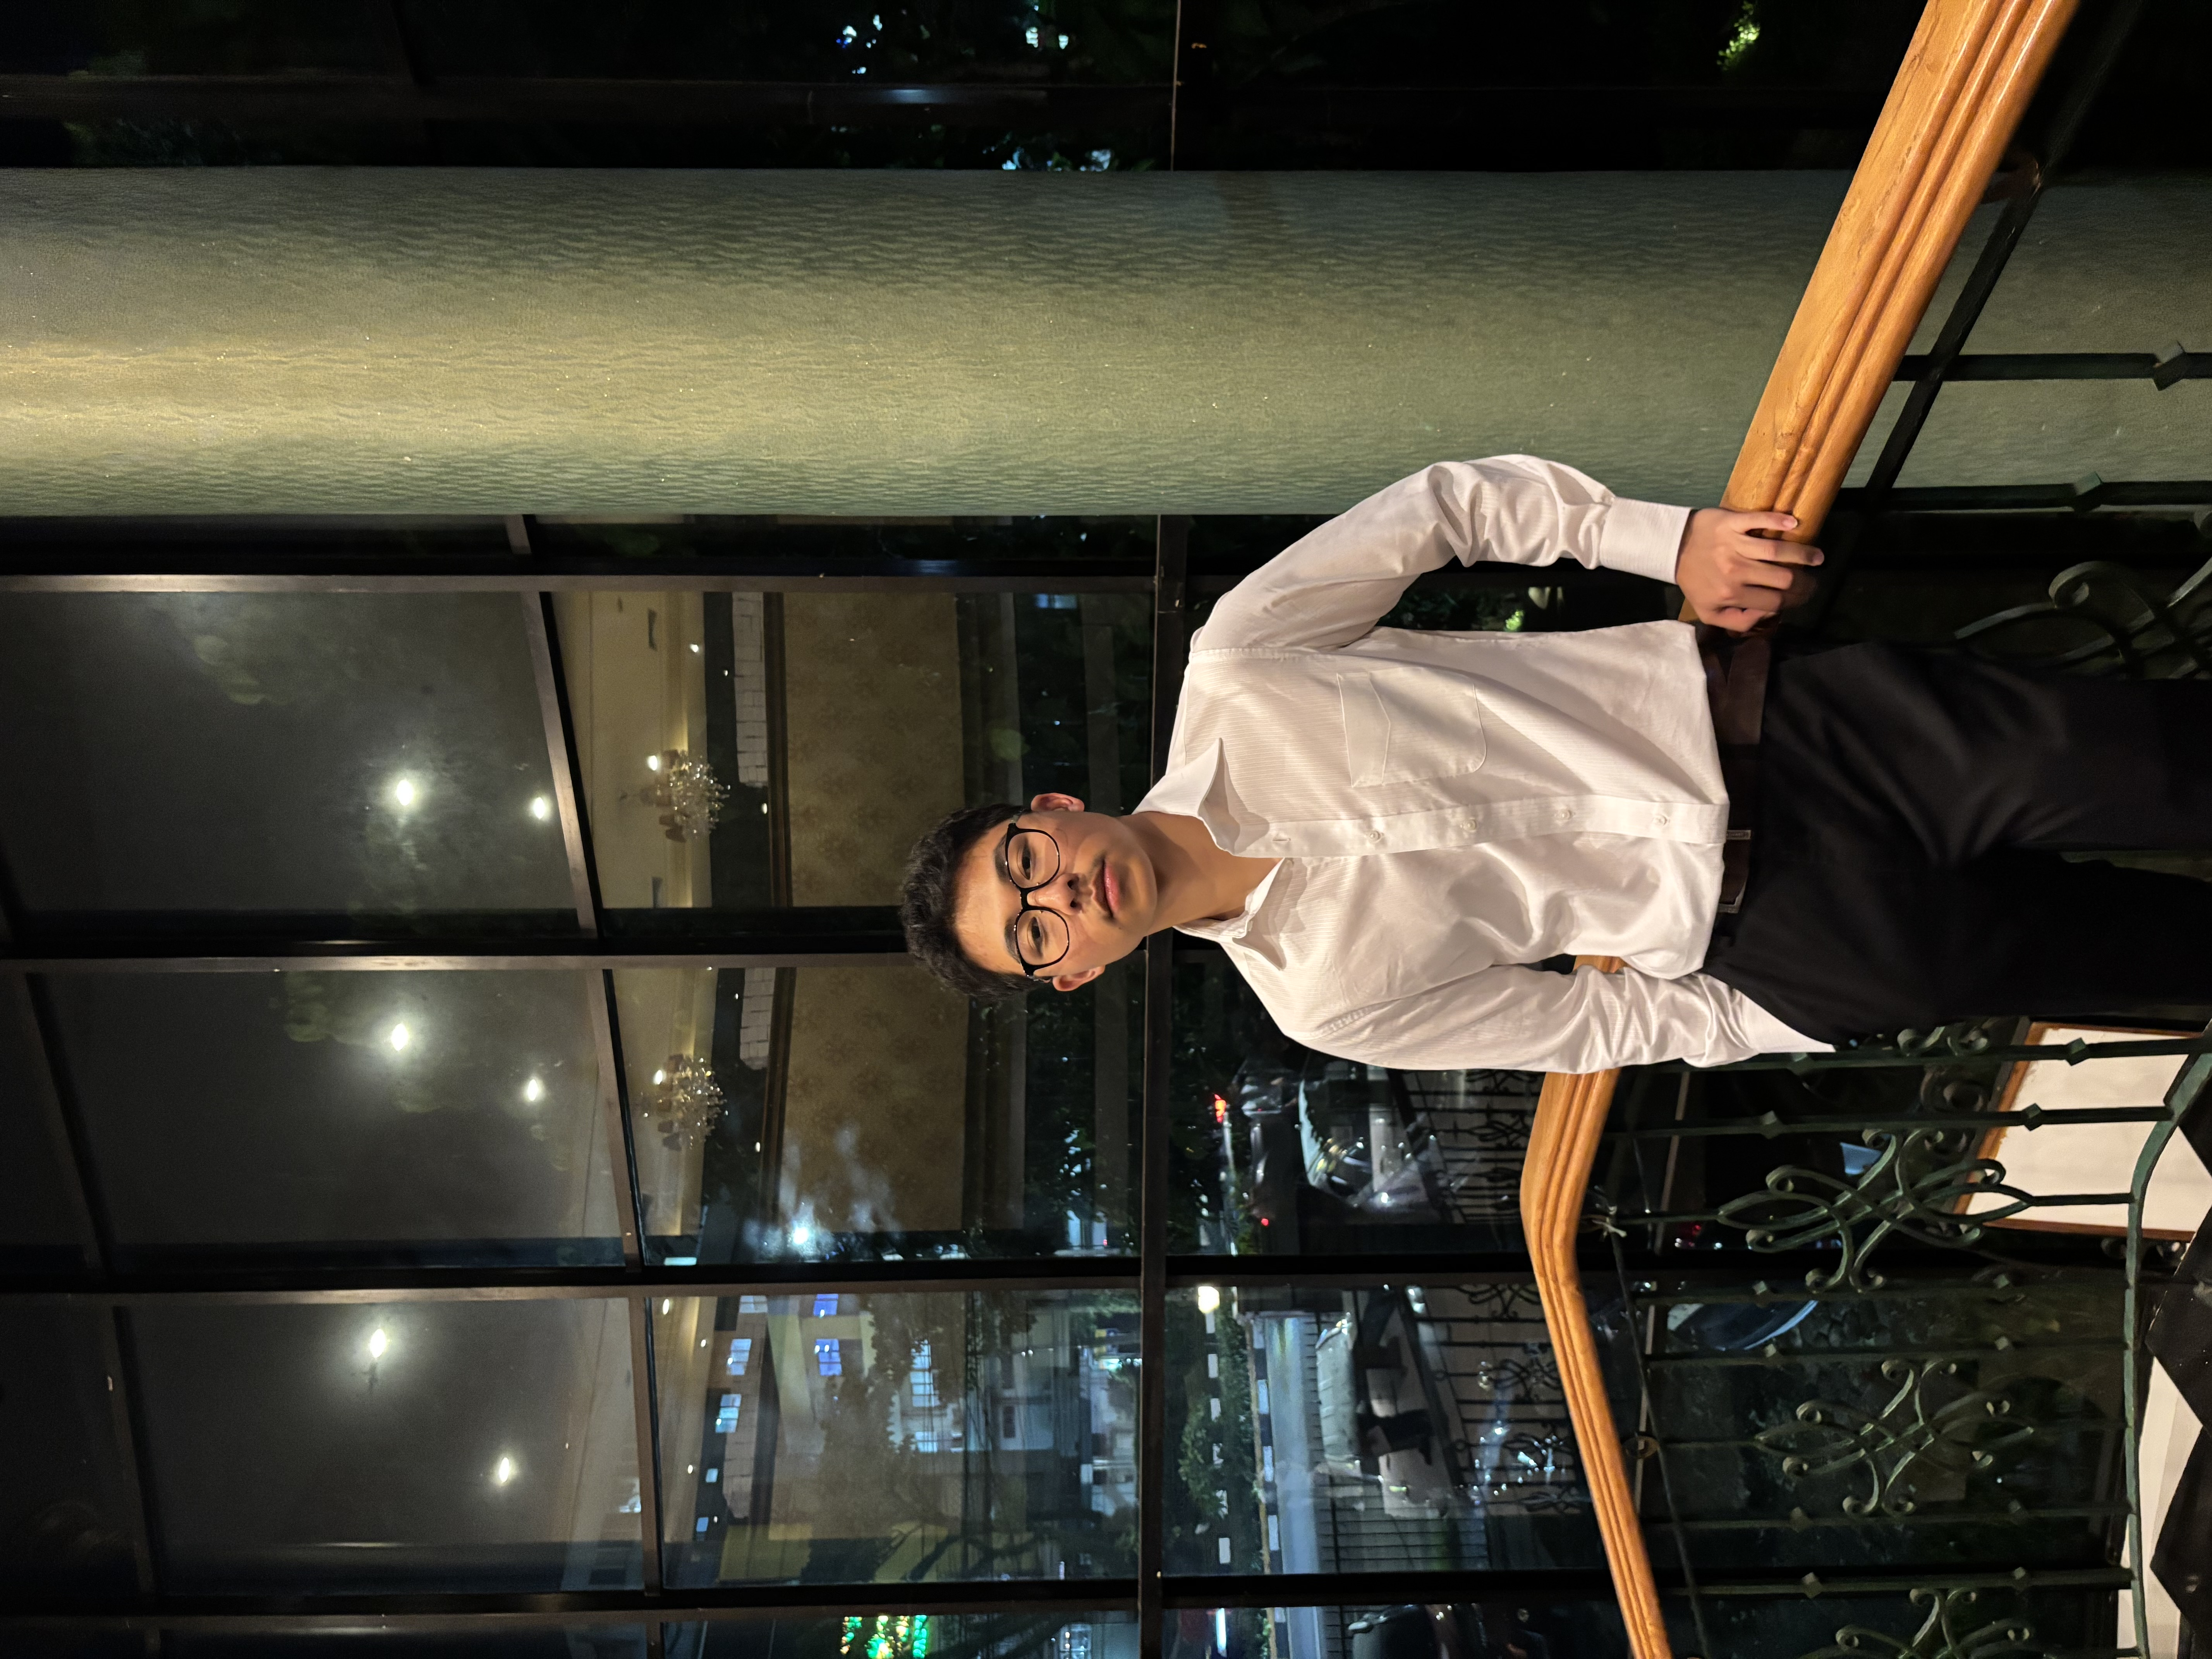
\includegraphics[width=1\linewidth,height=\textheight,keepaspectratio]{images/oks.jpg}

}

\caption{About Me}

\end{figure}%

Halo! Senang sekali Anda mampir!

Perkenalkan, saya Jonathan Kenan Budianto, atau panggil saja Kenan. Saya
adalah seorang pemimpi berusia 19 tahun dari Jakarta yang sedang memulai
salah satu petualangan paling seru dalam hidup: menjadi seorang
mahasiswa. Bagi saya, setiap hari adalah sebuah halaman baru yang siap
diisi dengan pembelajaran, tawa, dan tentu saja, cerita-cerita tak
terduga!

Saya tumbuh dalam kehangatan keluarga besar, di mana pintu rumah selalu
terbuka dan meja makan tak pernah sepi. Kakek dan nenek saya adalah
pahlawan saya; mereka mengajarkan sebuah pelajaran sederhana namun
sangat mendalam: bahwa kebaikan tidak mengenal batas, dan setiap orang
yang kita temui adalah bagian dari keluarga besar kita sendiri. Filosofi
inilah yang menjadi kompas hidup saya, sebuah pengingat untuk selalu
menyebarkan kepedulian dan membangun jembatan, bukan tembok.

Ada sebuah percikan semangat di dalam diri saya yang selalu menyala
paling terang ketika saya bisa menjadi bagian dari sesuatu yang lebih
besar. Saya sangat percaya pada kekuatan kolaborasi dan pemberdayaan.
Melihat sebuah ide tumbuh menjadi kenyataan, menyaksikan orang-orang di
sekitar saya mencapai potensi mereka, dan merasakan energi dari sebuah
komunitas yang bergerak bersama itulah yang membuat saya bersemangat!
Visi saya sederhana: menggunakan setiap ilmu dan karakter yang saya
miliki untuk ikut serta membangun masyarakat yang lebih baik, lebih
adil, dan lebih sinergis.

Di sini, di ruang digital kecil ini, saya ingin mengajak Anda untuk
melihat dunia melalui mata saya. Ini bukan sekadar portofolio; ini
adalah kumpulan fragmen perjalanan saya dari momen-momen penuh tawa,
pelajaran berharga, hingga impian-impian besar yang sedang saya kejar.

Jadi, mari kita mulai petualangan ini. Selamat menjelajah, dan saya
harap Anda menemukan sesuatu yang menginspirasi di sini!

\bookmarksetup{startatroot}

\chapter{UTS-1 All About Me}\label{uts-1-all-about-me}

Siapakah saya? Sebuah pertanyaan yang terdengar seperti awal dari esai
filsafat yang rumit. Tapi tenang, jawaban saya jauh lebih sederhana dan
melibatkan lebih banyak masakan enak. Bagi saya, Jonathan Kenan
Budianto, ``diri'' adalah sebuah resep yang terus disempurnakan, dengan
bahan-bahan utama yang saya dapatkan dari tempat paling hangat di muka
bumi: rumah kakek dan nenek.

\subsection{Akar yang Menumbuhkan: Pelajaran dari Rumah (dan
Dapur)}\label{akar-yang-menumbuhkan-pelajaran-dari-rumah-dan-dapur}

Fondasi cerita saya dibangun di rumah kakek dan nenek, sebuah tempat di
mana kepedulian adalah bumbu rahasia dalam setiap masakan. Di sanalah
saya belajar dua hal paling fundamental dalam hidup.

Pelajaran pertama datang dari nenek saya, seorang ahli diplomasi yang
menggunakan teh hangat dan kue sebagai ``senjata''-nya. Tidak ada kurir
atau tamu yang bisa lolos dari ``interogasi'' ramahnya. Dari beliau,
saya mendapatkan \textbf{wawasan mendalam} bahwa \textbf{empati bukanlah
sebuah teori, melainkan sebuah tindakan nyata} sesederhana memastikan
orang lain merasa dilihat dan dihargai, bahkan dalam interaksi sekecil
apa pun.

Pelajaran kedua, dari kakek saya, adalah tentang \textbf{humor sebagai
alat bertahan hidup paling ampuh}. Saya pernah melihatnya bersenandung
sambil membetulkan keran yang (untuk kesekian kalinya) bocor. Saya, yang
saat itu mungkin sedang stres karena masalah remaja yang sepele,
bertanya bagaimana beliau bisa sesantai itu. Beliau menepuk pundak saya,
menatap keran itu, lalu menatap saya, dan berkata dengan sangat serius,
``Karena kalau cemberut, kerannya tetap bocor, tapi wajah ganteng kakek
jadi ikut bocor.''

\subsection{Dari Ilmu ke Aksi: Kesenangan dalam ``Menggembalakan
Kucing''}\label{dari-ilmu-ke-aksi-kesenangan-dalam-menggembalakan-kucing}

Ada sebuah kepuasan yang tak ternilai ketika ilmu yang kita pelajari
bisa bertransformasi menjadi aksi nyata. Saya menemukan kebahagiaan itu
saat terlibat dalam berbagai kegiatan, mencoba menerapkan nilai-nilai
dari rumah dalam skala yang lebih besar.

Tentu saja, prosesnya tidak selalu mulus. Terkadang, upaya memberdayakan
sebuah tim lebih terasa seperti mencoba \textbf{menggembalakan kucing}
semua orang berlari ke arah yang berbeda dengan antusiasme
masing-masing. Namun, di dalam kekacauan itulah saya mendapatkan
\textbf{wawasan baru}: bahwa di situlah letak keindahan kolaborasi dan
kesabaran. Momen ketika ``kucing-kucing'' itu akhirnya berjalan ke arah
yang sama adalah sebuah kemenangan kecil yang sangat memuaskan.

\subsection{Visi ke Depan: Tetap Tersenyum pada Keran
Bocor}\label{visi-ke-depan-tetap-tersenyum-pada-keran-bocor}

Perjalanan ini masih panjang. Visi saya ke depan sederhana: terus
belajar, terus bertumbuh, dan terus memanfaatkan setiap kesempatan untuk
memberi dampak positif. Dan tentu saja, sambil berusaha mengingat
nasihat kakek untuk tidak cemberut pada ``keran-keran bocor'' dalam
hidup, karena itu hanya akan membuat masalahnya tetap sama, plus wajah
kita jadi kurang menarik.

Pada akhirnya, ``All About Me'' bukan hanya tentang siapa saya sekarang,
tetapi tentang siapa saya ingin menjadi: seseorang yang ceritanya bisa
membawa dampak baik, dan mungkin, sedikit tawa di sepanjang jalan.

\bookmarksetup{startatroot}

\chapter{UTS-2 Songs for You}\label{uts-2-songs-for-you}

Jika ada satu hal yang saya pelajari dari keluarga, itu adalah cinta.
Jika ada hal kedua, itu adalah bahwa bakat musik saya mungkin lebih
cocok untuk dinikmati\ldots{} sendirian di kamar mandi. Untungnya, ada
musisi seperti Tulus yang bisa meminjamkan suaranya untuk menceritakan
kisah yang tidak bisa saya nyanyikan.

\begin{center}\rule{0.5\linewidth}{0.5pt}\end{center}

\subsection{``Monokrom'' oleh Tulus}\label{monokrom-oleh-tulus}

\emph{Soundtrack Tidak Resmi Rumah Kakek dan Nenek.}

Saya tidak memilih lagu ini. Rasanya, lagu inilah yang menemukan saya.
Saat Tulus bernyanyi tentang \emph{``wangi rumah di sore itu, kue
cokelat dan susu''}, saya tidak sedang mendengarkan lirik; saya sedang
melancarkan kembali sebuah misi spionase masa kecil. Nama misi: Operasi
Kue Bolu. Target: kue buatan nenek yang baru keluar dari oven. Tingkat
keberhasilan: nol persen. Nenek selalu tahu, tapi beliau punya kebijakan
``pura-pura tidak lihat'' yang sangat saya hargai.

Lalu ada lirik \emph{``suaramu buatku lelap''}. Ini adalah ulasan paling
akurat untuk sesi dongeng sebelum tidur dari kakek saya. Ceritanya
mungkin tentang kancil yang cerdik melawan buaya, tapi efek suaranya
lebih manjur dari lagu nina bobo manapun. Saya yakin saya tertidur di
tengah-tengah plot twist paling menegangkan lebih sering daripada yang
bisa saya hitung.

Namun, di balik tawa dan aroma kue itu, lagu ini menyimpan sebuah
\textbf{wawasan yang mendalam}. Kakek dan nenek tidak hanya memberi kami
rumah untuk berteduh; mereka memberi kami ``warna'' dalam hidup warna
dari kehangatan, kepedulian, dan tawa yang menular. Lirik \emph{``Tak
akan ku mengenal cinta, bila bukan karena hati baikmu''} adalah
kebenaran inti yang menopang seluruh cerita saya.

Maka, \textbf{inspirasi} terbesar dari lagu ini bukanlah nostalgia
semata, melainkan sebuah janji. Janji untuk meneruskan ``warna'' itu.
Kini giliran saya untuk menjadi ``hati baik'' bagi orang lain,
memastikan kehangatan yang saya terima terus mengalir lengkap dengan
kebijakan ``pura-pura tidak lihat'' saat seseorang butuh sedikit
kebahagiaan ekstra.

\url{https://youtu.be/QqJ-Vp8mvbk?si=EwTS6Vq6e2jJM6FR}

\begin{quote}
\textbf{Lirik Lengkap ``Monokrom''}

Lembaran foto hitam putih

Aku coba ingat lagi warna bajumu kala itu

Kali pertama di hidupku

Manusia lain memelukku

Lembaran foto hitam putih

Aku coba ingat lagi wangi rumah di sore itu

Kue cokelat dan susu

Dan tiga bocah di selebar koran sore

Di mana pun kalian berada

Kukirimkan terima kasih

Untuk warna dalam hidupku dan banyak kenangan indah

Kau melukis aku

Lembaran foto hitam putih

Kembali teringat malam kuhitung-hitung bintang

Saat mataku sulit tidur

Suaramu buatku lelap

Di mana pun kalian berada

Kukirimkan terima kasih

Untuk warna dalam hidupku dan banyak kenangan indah

Kau melukis aku

Kita tak pernah tahu berapa lama kita diberi waktu

Jika aku pergi lebih dulu, jangan lupakan aku

Ini lagu untukmu, ungkapan terima kasihku

Lembar monokrom hitam putih

Aku coba ingat warna demi warna di hidupku

Tak akan ku mengenal cinta

Bila bukan karena hati baikmu
\end{quote}

\bookmarksetup{startatroot}

\chapter{UTS-3 My Stories for You}\label{uts-3-my-stories-for-you}

Terkadang, pelajaran hidup yang paling berharga tidak datang dari
buku-buku tebal, melainkan dari momen-momen kecil yang tak terduga.
Cerita berikut ini adalah salah satu momen itu sebuah pengingat tentang
dari mana saya berasal dan untuk apa saya berjuang.

\begin{center}\rule{0.5\linewidth}{0.5pt}\end{center}

\subsection{Pelajaran dari Kotak
Kardus}\label{pelajaran-dari-kotak-kardus}

Adik perempuan saya pulang dari sekolah dengan wajah murung. Di
tangannya ada secarik kertas tugas: membuat diorama ekosistem laut dari
bahan bekas. Bagi sebagian anak, ini mungkin tugas yang menyenangkan.
Tapi bagi adik saya yang saat itu merasa kurang percaya diri dengan
kemampuan seninya, tugas ini terasa seperti gunung yang mustahil didaki.

``Aku nggak bisa, Kak,'' keluhnya sambil meletakkan beberapa botol
plastik dan sebuah kotak kardus bekas di lantai. ``Pasti punya
teman-teman yang lain lebih bagus.''

Melihat keputusasaan di matanya, saya teringat akan pelajaran dari kakek
dan nenek: kepedulian terbesar sering kali hadir dalam bentuk waktu dan
perhatian. Saya pun duduk di sampingnya di lantai, di antara tumpukan
``sampah'' yang akan kami sulap. Saya tidak mengambil alih tugasnya.
Sebaliknya, saya hanya bertanya, ``Menurutmu, karang paling bagus dibuat
dari apa? Kalau ikan, bagaimana caranya agar bisa `berenang'?''

Selama tiga jam berikutnya, kami bekerja bersama. Saya membantunya
memotong bagian yang sulit, memberinya ide untuk membuat gurita dari
sisa benang wol, dan yang terpenting, meyakinkannya bahwa setiap
potongan yang ia tempel sudah sangat bagus. Perlahan, wajah murungnya
berubah menjadi senyum konsentrasi, lalu tawa bangga saat diorama itu
mulai terbentuk. Kotak kardus itu bukan lagi sekadar kotak kardus; ia
telah menjadi samudra penuh warna di ruang keluarga kami.

Esoknya, ia pulang dengan senyum yang jauh lebih lebar. Dioramanya
mendapat pujian dari guru. Tapi bukan itu kemenangannya. Kemenangan
sesungguhnya adalah kilau di matanya saat ia berkata, ``Kak, ternyata
aku bisa, ya?''

Momen itu mengajarkan saya sebuah pelajaran yang mendalam. Kebahagiaan
terbesar bukanlah saat kita mencapai sesuatu untuk diri kita sendiri,
tetapi saat kita bisa menjadi `percikan api' yang membantu orang lain
menemukan kekuatan dalam diri mereka. Pelajaran dari kotak kardus itu
terus saya bawa hingga hari ini, sebagai pengingat bahwa memberdayakan
orang lain adalah aktualisasi diri yang paling sejati.

\bookmarksetup{startatroot}

\chapter{UTS-4 My SHAPE}\label{uts-4-my-shape}

Memahami diri adalah langkah pertama untuk bisa memberi dampak. Analisis
SHAPE ini adalah proses saya memetakan dan menyatukan berbagai kepingan
yang membentuk identitas saya. Ini bukan sekadar daftar, melainkan
sebuah kompas yang saya susun untuk menavigasi perjalanan hidup,
memastikan setiap langkah selaras dengan panggilan hati saya.

\begin{center}\rule{0.5\linewidth}{0.5pt}\end{center}

\subsection{Peta SHAPE Saya}\label{peta-shape-saya}

\begin{itemize}
\tightlist
\item
  \textbf{S -- Strengths (Kekuatan Khas):}

  \begin{itemize}
  \tightlist
  \item
    \textbf{Empati:} Kemampuan untuk merasakan dan memahami perspektif
    orang lain, sebuah kekuatan yang ditanamkan sejak kecil oleh
    keluarga.
  \item
    \textbf{Pengembangan Orang Lain:} Menemukan energi dan kepuasan saat
    membantu orang lain bertumbuh dan menemukan potensi mereka.
  \item
    \textbf{Pemikiran Kritis \& Reflektif:} Kemampuan untuk menganalisis
    keadaan dan secara sadar merenungkan proses pengembangan diri untuk
    menjadi lebih baik.
  \item
    \textbf{Kepemimpinan Melayani:} Memimpin dengan memberi dukungan dan
    menciptakan lingkungan di mana setiap orang merasa dihargai dan bisa
    berkontribusi.
  \end{itemize}
\item
  \textbf{H -- Heart (Panggilan Hati):}

  \begin{itemize}
  \tightlist
  \item
    \textbf{Pemberdayaan Komunitas:} Hati saya terpanggil untuk terlibat
    dalam upaya menjadikan lingkungan sekitar menjadi lebih baik,
    sinergis, dan ideal.
  \item
    \textbf{Keadilan \& Kepedulian:} Sebuah hasrat mendalam untuk
    memastikan setiap individu, terlepas dari latar belakangnya,
    diperlakukan dengan baik dan menjadi bagian dari ``keluarga''.
  \item
    \textbf{Pertumbuhan Bersama:} Saya sangat percaya pada kekuatan
    kolaborasi dan sinergi; kita tumbuh paling kuat saat kita tumbuh
    bersama.
  \end{itemize}
\item
  \textbf{A -- Aptitudes \& Acquired Skills (Bakat \& Keterampilan):}

  \begin{itemize}
  \tightlist
  \item
    \textbf{Komunikasi Interpersonal:} Terlatih untuk mendengarkan dan
    membangun hubungan yang tulus, berkat lingkungan keluarga yang
    sangat komunal.
  \item
    \textbf{Manajemen Organisasi:} Memiliki kemampuan untuk mengelola
    kegiatan dan memberdayakan tim untuk mencapai tujuan bersama.
  \item
    \textbf{Fasilitasi dan Mentoring:} Mampu memandu dan mendukung orang
    lain dalam proses belajar dan pengembangan diri mereka.
  \end{itemize}
\item
  \textbf{P -- Personality (Gaya Kepribadian):}

  \begin{itemize}
  \tightlist
  \item
    \textbf{Kolaboratif:} Saya bekerja paling efektif saat berada dalam
    tim, berbagi ide, dan membangun sesuatu bersama-sama.
  \item
    \textbf{Berorientasi pada Orang Lain (People-Oriented):} Fokus saya
    secara alami tertuju pada kesejahteraan dan pertumbuhan orang-orang
    di sekitar saya.
  \item
    \textbf{Reflektif \& Introspektif:} Saya cenderung mengambil waktu
    untuk merenung dan memahami ``mengapa'' di balik setiap tindakan dan
    tujuan.
  \end{itemize}
\item
  \textbf{E -- Experiences (Pengalaman Kunci):}

  \begin{itemize}
  \tightlist
  \item
    \textbf{Pelajaran dari Keluarga Besar:} Dibesarkan di lingkungan
    yang mengutamakan kebersamaan dan kepedulian telah menjadi
    pengalaman formatif yang membentuk seluruh pandangan dunia saya
    tentang hubungan antarmanusia.
  \item
    \textbf{Terlibat dalam Pemberdayaan Lingkungan:} Setiap momen di
    mana saya bisa berkontribusi dalam kegiatan yang memberdayakan
    komunitas telah mengkonfirmasi panggilan hati saya dan memberikan
    kepuasan yang mendalam.
  \end{itemize}
\end{itemize}

\begin{center}\rule{0.5\linewidth}{0.5pt}\end{center}

\subsection{Piagam Diri (Self-Charter)}\label{piagam-diri-self-charter}

\textbf{Misi Hidup Saya:} \textgreater{} Menjadi katalisator kebaikan,
menggunakan empati dan semangat kolaborasi untuk membangun komunitas di
mana setiap individu merasa berdaya, dihargai, dan terinspirasi untuk
bertumbuh.

\textbf{Nilai Inti Saya:} \textgreater{} Empati, Kepedulian, Kolaborasi,
Pertumbuhan, dan Integritas.

\textbf{Janji Pelayanan Saya:} \textgreater{} Saya berjanji untuk selalu
hadir dengan telinga yang mendengar, hati yang peduli, dan tangan yang
siap membantu, menciptakan ruang yang aman bagi orang lain untuk menjadi
versi terbaik dari diri mereka.

\begin{center}\rule{0.5\linewidth}{0.5pt}\end{center}

\subsection{Narasi 90 Detik (Elevator
Pitch)}\label{narasi-90-detik-elevator-pitch}

``Halo, saya Kenan. Saya adalah seorang pembelajar dan pemberdaya yang
percaya bahwa perubahan terbesar dimulai dari kepedulian tulus.
Dibesarkan dalam keluarga yang mengajarkan bahwa semua orang adalah
bagian dari kita, saya membawa nilai empati dalam segala hal. Kekuatan
saya terletak pada kemampuan untuk menghubungkan orang dan membantu
mereka bertumbuh bersama. Hati saya terpanggil untuk membangun komunitas
yang sinergis dan ideal. Dengan pengalaman dalam memfasilitasi dan
berorganisasi, misi saya sederhana: mencapai aktualisasi diri dengan
cara memberdayakan orang-orang di sekitar saya.''

\bookmarksetup{startatroot}

\chapter{UTS-5 My Personal Review}\label{uts-5-my-personal-review}

Selamat datang di tahap refleksi. Bagian ini adalah wujud dari keyakinan
saya bahwa pertumbuhan sejati lahir dari evaluasi yang jujur dan kritis.
Sesuai dengan instruksi tugas, halaman ini berisi dua jenis asesmen
terhadap karya UTS-1 hingga UTS-4:

\begin{enumerate}
\def\labelenumi{\arabic{enumi}.}
\tightlist
\item
  \textbf{Self-Assessment:} Sebuah tinjauan mendalam yang dilakukan
  untuk menganalisis kekuatan dan area pengembangan dari karya saya
  sendiri.
\item
  \textbf{Peer-Assessment:} Tinjauan konstruktif yang dilakukan secara
  manual terhadap karya tiga rekan mahasiswa.
\end{enumerate}

Hasil kuantitatif dari semua penilaian ini dirangkum dalam Lembar Skor
yang dapat diakses di bagian akhir halaman ini.

\begin{center}\rule{0.5\linewidth}{0.5pt}\end{center}

\subsection{1. Self-Assessment}\label{self-assessment}

Berikut adalah hasil penilaian terhadap portofolio saya sendiri.

\subsubsection{1.1 Tinjauan Umum \& Skor
Rinci}\label{tinjauan-umum-skor-rinci}

Secara keseluruhan, portofolio ini menunjukkan kualitas pengerjaan yang
sangat tinggi, dengan narasi personal yang konsisten, mendalam, dan
menyentuh di seluruh tugas. Tema utama yang diangkat adalah nilai-nilai
yang ditanamkan oleh keluarga, seperti empati, kepedulian, humor, dan
semangat untuk memberdayakan orang lain.

\begin{itemize}
\tightlist
\item
  \textbf{UTS-1 (All About Me):}

  \begin{itemize}
  \tightlist
  \item
    \textbf{Tinjauan:} Halaman ini secara efektif memperkenalkan diri
    melalui cerita personal tentang pelajaran yang didapat dari kakek
    dan nenek.
  \item
    \textbf{Skor:} Orisinalitas (5), Keterlibatan (5), Humor (5),
    Wawasan (5) → \textbf{Total: 20/20}
  \end{itemize}
\item
  \textbf{UTS-2 (Songs for You):}

  \begin{itemize}
  \tightlist
  \item
    \textbf{Tinjauan:} Memilih lagu ``Monokrom'' dari Tulus dan
    mengikatnya dengan sangat kuat pada kenangan personal bersama
    keluarga.
  \item
    \textbf{Skor:} Orisinalitas (5), Keterlibatan (5), Humor (4),
    Inspirasi (5) → \textbf{Total: 19/20}
  \end{itemize}
\item
  \textbf{UTS-3 (My Stories for You):}

  \begin{itemize}
  \tightlist
  \item
    \textbf{Tinjauan:} Kisah ``Pelajaran dari Kotak Kardus'' adalah
    sebuah cerita yang indah tentang pemberdayaan.
  \item
    \textbf{Skor:} Orisinalitas (5), Keterlibatan (5), Pengembangan
    Narasi (5), Inspirasi (5) → \textbf{Total: 20/20}
  \end{itemize}
\item
  \textbf{UTS-4 (My SHAPE):}

  \begin{itemize}
  \tightlist
  \item
    \textbf{Tinjauan:} Menyajikan analisis SHAPE yang terstruktur dengan
    baik, lengkap dengan Peta SHAPE, Piagam Diri, dan Narasi 90 Detik.
  \item
    \textbf{Skor:} Orisinalitas (5), Keterlibatan (5), Pengembangan
    Narasi (5), Inspirasi (5) → \textbf{Total: 20/20}
  \end{itemize}
\end{itemize}

\subsubsection{1.2 Penilaian UTS-5 (Self-Assessment
ini)}\label{penilaian-uts-5-self-assessment-ini}

\begin{itemize}
\tightlist
\item
  \textbf{Skor per kriteria:} Pemahaman Konsep (5), Analisis Kritis (5),
  Argumentasi (5), Etos \& Empati (5), Rekomendasi (5) → \textbf{Total
  25/25 (100\%).}
\item
  \textbf{Alasan singkat:} Telah berhasil memenuhi tugas
  \emph{Self-Assessment} dengan melakukan telaah kritis yang tajam dan
  memberikan rekomendasi perbaikan yang konkret dan aplikatif untuk
  setiap bagian.
\end{itemize}

\subsubsection{1.3 Saran Perbaikan untuk Diri
Sendiri}\label{saran-perbaikan-untuk-diri-sendiri}

\begin{itemize}
\tightlist
\item
  \textbf{UTS-2 (Refleksi Musik):} Bisa ditambahkan satu kalimat
  refleksi tentang bagaimana musik secara umum menjadi cara saya
  memproses kenangan untuk memperdalam narasi.
\end{itemize}

\begin{center}\rule{0.5\linewidth}{0.5pt}\end{center}

\subsection{2. Peer-Assessment}\label{peer-assessment}

Berikut adalah hasil penilaian terhadap portofolio rekan-rekan
mahasiswa. Penilaian dilakukan berdasarkan rubrik UTS-1 hingga UTS-4.

\subsubsection{2.1 Penilaian untuk: M. Abizzar Gamadrian
(13523155)}\label{penilaian-untuk-m.-abizzar-gamadrian-13523155}

\begin{itemize}
\tightlist
\item
  \textbf{URL Portofolio:}
  \url{https://abizzarg.github.io/all-about-me/}
\item
  \textbf{Tinjauan Umum:} Portofolio Abizzar menunjukkan kualitas yang
  sangat tinggi dengan narasi personal yang kuat dan otentik. Tema utama
  tentang pencarian makna, ketangguhan, dan komitmen pada pertumbuhan
  diri terjalin dengan sangat baik di setiap tugas.
\item
  \textbf{Rincian Skor \& Saran:}

  \begin{itemize}
  \tightlist
  \item
    \textbf{UTS-1 (Skor: 19/20):} Orisinalitas (5), Keterlibatan (5),
    Humor (4), Wawasan (5). Kualitas sudah sangat tinggi. Penambahan
    satu anekdot singkat bisa lebih memperkuat sisi humor.
  \item
    \textbf{UTS-2 (Skor: 15/20):} Orisinalitas (4), Keterlibatan (4),
    Humor (2), Inspirasi (5). Narasi personal sebelum lirik bisa
    diperluas untuk menceritakan ``mengapa'' lagu ini begitu penting,
    sehingga meningkatkan skor keterlibatan.
  \item
    \textbf{UTS-3 (Skor: 20/20):} Orisinalitas (5), Keterlibatan (5),
    Pengembangan Narasi (5), Inspirasi (5). Sempurna. Sebuah contoh
    penceritaan yang sangat baik.
  \item
    \textbf{UTS-4 (Skor: 20/20):} Orisinalitas (5), Keterlibatan (5),
    Pengembangan Narasi (5), Inspirasi (5). Sebuah contoh analisis diri
    yang luar biasa.
  \end{itemize}
\end{itemize}

\subsubsection{2.2 Penilaian untuk: Muhammad
Syafiq}\label{penilaian-untuk-muhammad-syafiq}

\begin{itemize}
\tightlist
\item
  \textbf{URL Portofolio:}
  \url{https://iammadsfq.github.io/all-about-me/}
\item
  \textbf{Tinjauan Umum:} Portofolio ini menyajikan sebuah narasi yang
  tulus dan reflektif. Penulis berhasil membangun cerita yang konsisten
  tentang perjalanan diri, menyoroti pentingnya nilai-nilai, pengalaman,
  dan tujuan hidup.
\item
  \textbf{Rincian Skor \& Saran:}

  \begin{itemize}
  \tightlist
  \item
    \textbf{UTS-1 (Skor: 14/20):} Orisinalitas (4), Keterlibatan (4),
    Humor (2), Wawasan (4). Saran: Tambahkan satu anekdot lucu yang
    relevan untuk meningkatkan Keterlibatan dan Humor.
  \item
    \textbf{UTS-2 (Skor: 15/20):} Orisinalitas (3), Keterlibatan (4),
    Humor (N/A), Inspirasi (4). Saran: Ceritakan sebuah momen spesifik
    di mana lagu tersebut menjadi \emph{soundtrack} hidup Anda untuk
    memperkuat Orisinalitas.
  \item
    \textbf{UTS-3 (Skor: 19/20):} Orisinalitas (5), Keterlibatan (5),
    Pengembangan Narasi (4), Inspirasi (5). Saran: Pastikan ada puncak
    (klimaks) cerita yang jelas sebelum menuju resolusi untuk
    menyempurnakan Pengembangan Narasi.
  \item
    \textbf{UTS-4 (Skor: 19/20):} Orisinalitas (5), Keterlibatan (4),
    Pengembangan Narasi (5), Inspirasi (5). Saran: Awali setiap bagian
    SHAPE dengan cerita singkat untuk membuat konten lebih naratif dan
    memikat.
  \end{itemize}
\end{itemize}

\subsubsection{2.3 Penilaian untuk: Jonathan
W}\label{penilaian-untuk-jonathan-w}

\begin{itemize}
\tightlist
\item
  \textbf{URL Portofolio:}
  \url{https://jonathanw33.github.io/all-about-me/}
\item
  \textbf{Tinjauan Umum:} Portofolio ini menunjukkan kualitas pengerjaan
  yang sangat tinggi, dengan narasi personal yang konsisten, mendalam,
  dan menyentuh di seluruh tugas. Tema utama tentang nilai-nilai
  keluarga (empati, humor, kepedulian) terjalin dengan sangat baik.
\item
  \textbf{Rincian Skor \& Saran:}

  \begin{itemize}
  \tightlist
  \item
    \textbf{UTS-1 (Skor: 19/20):} Orisinalitas (5), Keterlibatan (5),
    Humor (4), Wawasan (5). Kualitas sudah sangat baik. Humor bisa lebih
    merata di sepanjang narasi untuk mencapai skor sempurna.
  \item
    \textbf{UTS-2 (Skor: 18/20):} Orisinalitas (4), Keterlibatan (5),
    Humor (4), Inspirasi (5). Untuk meningkatkan orisinalitas, bisa
    ditambahkan refleksi tentang bagaimana elemen musik dari lagu itu
    sendiri memperkuat kenangan.
  \item
    \textbf{UTS-3 (Skor: 20/20):} Orisinalitas (5), Keterlibatan (5),
    Pengembangan Narasi (5), Inspirasi (5). Sempurna. Sebuah contoh
    penceritaan yang luar biasa.
  \item
    \textbf{UTS-4 (Skor: 19/20):} Orisinalitas (5), Keterlibatan (4),
    Pengembangan Narasi (5), Inspirasi (5). Untuk meningkatkan
    keterlibatan, pertimbangkan mengubah beberapa daftar poin menjadi
    paragraf naratif singkat.
  \end{itemize}
\end{itemize}

\begin{center}\rule{0.5\linewidth}{0.5pt}\end{center}

\subsection{Unduh Lembar Skor Lengkap}\label{unduh-lembar-skor-lengkap}

Semua skor kuantitatif dari asesmen yang dilakukan telah saya rekam
dalam format CSV sesuai template yang diberikan.

\href{./UTS-5_Skor.csv}{\textbf{1. Unduh Lembar Skor (Self + Peer)}}

\href{./Self-Assessment_UTS-1_s_d__UTS-5__dibuat_otomatis_.csv}{\textbf{2.
Unduh Rekap Self-Assessment (Format Otomatis)}}

\bookmarksetup{startatroot}

\chapter{UAS-1 My Concepts}\label{uas-1-my-concepts}

Mau hidup epik ? \href{lifestory.pdf}{Write your Life Story}

Apa itu berkonsep?

\url{https://youtu.be/QVfUlVBO80U?si=yM6q_rwV9rcDBbu7}

\bookmarksetup{startatroot}

\chapter{UAS-3 My Opinions}\label{uas-3-my-opinions}

SApa itu beropini? \href{BM\%20Opini.mp4}{Opini Berpengaruh}

Bagiamana menjaadi menarik? \href{./Interesting.mp4}{Menjadi Menarik}

\bookmarksetup{startatroot}

\chapter{UAS-3 My Innovations}\label{uas-3-my-innovations}

\bookmarksetup{startatroot}

\chapter{UAS-4 My Knowledge}\label{uas-4-my-knowledge}

Cara saya mengkomunikasikan sebuah pengatahuan sebagai petunjuk bagi
orang lain 1) saya tulis
\href{Rekomendasi\%20Presentasi\%20Efektif(Contoh\%20Makalah).pdf}{makalah
sebagai bahan utama} 2) lalu saya buat
\href{Contoh\%20Transkrip\%20Presentasi.pdf}{transkrip ucapan lisan} 3)
kemudian saya kembangkan
\href{Rekomendasi\%20Presentasi\%20(Contoh\%20Slides).pdf}{slide
pendukung trnsskrip} 4) lalu saya memproduksivideo audio visual
\url{https://youtu.be/ZbghfMvnPZc} \url{https://youtu.be/ZbghfMvnPZc}

\bookmarksetup{startatroot}

\chapter{UAS-5 My Professional
Reviews}\label{uas-5-my-professional-reviews}

Untuk melAkukan review, seperti pada
\href{../My_Personal_Reviews/Doc.5.Mengevaluasi-Esai-Berdasarkan-Rubrik.pdf}{pendekatan
AI}, kita membutuhkan rubrik

\bookmarksetup{startatroot}

\chapter{Summary}\label{summary}

In summary, this book has no content whatsoever.

\bookmarksetup{startatroot}

\chapter*{References}\label{references}
\addcontentsline{toc}{chapter}{References}

\markboth{References}{References}

\phantomsection\label{refs}




\end{document}
